The weak phase \phis is an important parameter of the \BBbarSyst system. It is related to the third
type of CP-Violation mentioned in \secref{Phenomenology}, nameley in the interference between
two decay amplitudes, see \figref{interference}. In the current section \phis and its relevance to
the search for new particles is discussed.

\newcommand{\ffig}{f}
\newcommand{\phimixfig}{\phi_\text{mix}}
\newcommand{\phifig}{\phi_\text{dec}}
\newcommand{\phibarfig}{\kern 0.15em \overline{\kern -0.15em \phi_\text{dec} \kern -0.60em} \kern 0.60em}
\begin{figure}[h]
  \centering
  \resizebox{0.4\textwidth}{!}{\begin{picture}(0,0)%
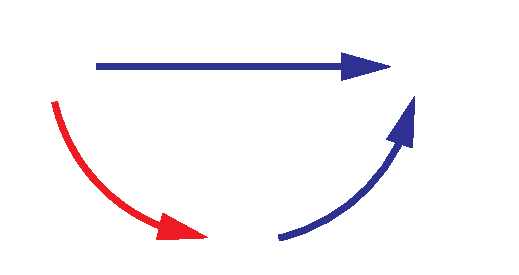
\includegraphics{Figures/Chapter1/decay_CMYK.pdf}%
\end{picture}%
\setlength{\unitlength}{4144sp}%
%
\begingroup\makeatletter\ifx\SetFigFont\undefined%
\gdef\SetFigFont#1#2#3#4#5{%
  \reset@font\fontsize{#1}{#2pt}%
  \fontfamily{#3}\fontseries{#4}\fontshape{#5}%
  \selectfont}%
\fi\endgroup%
\begin{picture}(3939,2094)(2644,-2188)
\put(3286,-736){\makebox(0,0)[rb]{\smash{{\SetFigFont{25}{30.0}{\sfdefault}{\mddefault}{\updefault}{\color[rgb]{0,0,0}$\Bs$}%
}}}}
\put(5761,-736){\makebox(0,0)[lb]{\smash{{\SetFigFont{25}{30.0}{\sfdefault}{\mddefault}{\updefault}{\color[rgb]{0,0,0}$\ffig$}%
}}}}
\put(4501,-421){\makebox(0,0)[b]{\smash{{\SetFigFont{25}{30.0}{\sfdefault}{\mddefault}{\updefault}{\color[rgb]{0,0,1}}%
}}}}
\put(5581,-1771){\makebox(0,0)[lb]{\smash{{\SetFigFont{25}{30.0}{\sfdefault}{\mddefault}{\updefault}{\color[rgb]{0,0,1}}%
}}}}
\put(3331,-1771){\makebox(0,0)[rb]{\smash{{\SetFigFont{25}{30.0}{\sfdefault}{\mddefault}{\updefault}{\color[rgb]{1,0,0}}%
}}}}
\put(4501,-2041){\makebox(0,0)[b]{\smash{{\SetFigFont{25}{30.0}{\sfdefault}{\mddefault}{\updefault}{\color[rgb]{0,0,0}$\Bsb$}%
}}}}
\end{picture}%
}
  \caption{The two interfering decay amplitudes leading to the same final state.
           The phases $\phimixfig$, $\phifig$ correspond to ....
           % This is assuming no CP violation in mixing or CP violation in decay.}
           }
  \label{interference}
\end{figure}

The parameter \phis manifests in the so called $\bquark \rightarrow \cquark\cquarkbar\squark $ transitions, where the
\bquark quuark of the \Bs meson decays into three other quarks. In addtion, the final state of the \Bs meson has to be
a CP eigenstate, which implies that both \Bs and \Bsb can decay into it, such that the two decay amplitudes of \figref{interference}
can interfere.

A common way to parametrize CP violation in the interference between mixing and decay is shown in \equref{lambda_cpv}
\footnote{This $\lambda_f$ is not to be confused with the $\lambda$ of the WOlfenstein Prametrization.}.

\begin{equation}
 \lambda_{f} = \eta_f \frac{q}{p} \frac{\bar{A}_f}{A_f}. % \equiv \left|\lambda_f\right| e^{i\phis}.
\label{lambda_cpv}
\end{equation}

\noindent The ratios $|\qoverp|$ and $|\nicefrac{A_f}{\bar{A}_{f}}|$ are ascociated to the mixing and decay parts of \figref{interference} respectivelly.
Whereas $\eta_f$ is the CP eigenvalue of the final state $f$ and can be either $+1$ or $-1$ corresponding to CP-even and CP-odd respectivelly.
The above parameter $\lambda_f$ is also releated to the $\Acp{\rm mix}$ and $\Acp{\rm dir}$ as it can be seen in {\color{red}  simple ref to that}.
Given the so called {\it master equations}{\color{red} ref pdg} for the decay rates of a \Bs and \Bsb
to a final state $f$, the \CP asymmetry due to the interference between mixing and decay\footnote{assuming $|\qoverp|=1$ and $|\nicefrac{A_f}{\bar{A}_{\bar{f}}}| = 1$ consistet with {\color{red} ref for nocpv in mix and decay}.}
is shown in \equref{cpv_interf}

\newcommand{\half}{\frac{1}{2}}
\begin{equation}
  \Acp{\text{inter}}(t) = \frac{ - \Im(\lambda_f) \sin(\Delta m_s t)} {\cosh(\half \Delta\Gamma_s t) - \Re(\lambda_f)\sinh(\half\Delta\Gamma_s t)}.
\label{cpv_interf}
\end{equation}

\noindent It is intreasting to point out that according to \equref{cpv_interf} CP asymmetry can still be observed in the interference between decay and
mixing even if no CP-Violation occurs in both the mixing and decay. This is posible if the overal phase of $\lambda_f$ in \equref{lambda_cpv} is not zero.
The asymmetry of \equref{cpv_interf} can vanish at a particular point of time or for a given time interval. Because of that \equref{lambda_cpv} should not
be integrated over time when measuring \phis. Impling that the time interval between the production and decay of a \Bs (\Bsb) meson has to be
known\footnote{This interval is called {\it decay time}.}.

\begin{figure}[h]
  \centering
  {\sffamily \input{Figures/Chapter1/tree}}
  \caption{{\color{red} Fix this to look more like \figref{QuarkMixing} and put ckm elements on the vertices}. Explain tha this is called tree diagram}
  \label{bs2jpsiphi}
\end{figure}

Given a certain final state $f$ \equref{lambda_cpv} can be expresed as a combination of CKM elements and thus obtain the
Standard Model estimate of $\Im(\lambda_f)$. The two mesons $\jpsi$ and $\phi$ is a typical choice for $f$ for reasons that are
explained later in this section. The leading order diagrams for the \BsJpsiPhi decay and the \BBbarSyst mixing are
shown in \figref{bs2jpsiphi} and \figref{bs_box} repsectivelly. From those diagrams the ratios $\qoverp$ and $\nicefrac{A_f}{\bar{A}_{f}}$
can be read as shown in \equref{qoverp}\footnote{Here it has been used {\color{red} equation blah from pdg} } and \equref{af_afbar} repsectivelly.

\begin{equation}
 \frac{q}{p} = \frac{\Vtb^*\Vts}{\Vtb\Vts^*}
\label{qoverp}
\end{equation}

\begin{equation}
 \frac{\bar{A}_{\jpsi\phi}} {A_{\jpsi\phi}} = \frac{\Vcb\Vcs^*}{\Vcb^*\Vcs}
\label{af_afbar}
\end{equation}

\noindent Combining \equref{qoverp}, \equref{af_afbar} and using the $\beta_s$ angle definition frm \equref{bsAnglesDef} the imaginary part of
$\lambda_{f}$ of \equref{lambda_cpv} is can be computed, see \equref{phis_def}\footnote{Based on the fact that for a complex number's argument, $\argu{z}$ it is: $\argu{z^{-1}}=\argu{-z}=\argu{z^*}=-\argu{z}$}.

\begin{align}
  \centering
 \Im(\lambda_f) =& \eta_f\sin\parenthesis{ \argu{\frac{\Vtb^*\Vts}{\Vtb\Vts^*}} + \argu{\frac{\Vcb\Vcs^*}{\Vcb^*\Vcs}} } \nonumber \\
                =& \eta_f\sin\parenthesis{ \argu{\parenthesis{\Vtb^*\Vts}^2}    + \argu{\frac{1}{\parenthesis{\Vcb^*\Vcs}^2}} }
                = \eta_f\sin\parenthesis{  2 \; \argu{\frac{\Vtb^*\Vts}{\Vcb^*\Vcs}} } \nonumber \\
                =& \sin\parenthesis{-2\betas}
                \equiv \eta_f\sin\parenthesis{\phis}
 \label{phis_def}
\end{align}

\noindent An additional implication arises from the choice of the $\jpsi\phi$ as the final state.
Specifically due to the fact that the last particles have a non zero spin quantum number, their combined wavefunction
is not a pure cp eigenstate. The eigenvalue $\eta_f$ of the last wavefunction dependants on the total angular momentum
$l$ of the $\jpsi$ and $\phi$ mesons. This dependancy has to be taken into acount in \equref{phis_def} resulting in \equref{phis_jpsiphi_def}

\begin{equation}
 \Im(\lambda_{\jpsi\phi}) = (-1)^l\sin\parenthesis{\phis}
 \label{phis_jpsiphi_def}
\end{equation}

\subsubsection{New Physics effects in \phis}

\begin{itemize}
 \item How NP effects can manifest in \phis (loop diagrams), Zprime
 \item Why does \phis has to be monitored
\end{itemize}

{\color{red} Put some new physics models and explain the flavor puzzle a bit. and why it is important to monitor \phis}

We measure

\begin{equation}
 \phis^{\text {eff}} = \phis^{\tiny \text{SM}} + \Delta\phis^{\tiny \text{NP}}
 \label{phis_meas}
\end{equation}

\subsubsection{Measuring \phis with the \lhcb detector}
The parameter \phis has been measuremed in the \lhcb experiment by analysing the decays of \BsJpsiPhi {\color{red} ref 3fb papaer}.
The particular choise of the last final state, where \phiKK and \Jpsimumu, was to do with several reasons. First the high number
of selected \BsJpsiPhi decays available at \lhcb, roughly $90$k at the end of the \runtwo is an advantage. Second it is relatively easy
to select real $\phi$ over other mesons that decay to a $K^+K^-$ pair. This is due to the fact that the $\phi$ meson dominates the
$K^+K^-$ mass distribution within a window of about $\pm 70 \mevcc$ around its mass. The last allows for the analysis to be
independant\footnote{There is some residual dependance left, which is very similar to what is described in \secref{Kpi_Invariant_mass}. }
of the \mkk mass variable and thus much simpler. However an angular analysis, see \secref{Diferential_Decay_Rate} is necessary
to disentangle the odd and even CP components of the final state $\jpsi\phi$, as it became apparent in \equref{phis_jpsiphi_def}.
In addition, as it was already implied \phis can be correctly probed only when the time dependance of the \BsJpsiPhi decays is taken into
account\footnote{Specifically \phis is the amplitude of the $\ket{\Bs{}_{,H}}$ and $\ket{\Bs{}_{,L}}$ time distribution oscilations
mentioned in and shown in {\color{red} ref to something.} }.
Furthermore knowledge on wheather the final state $\jpsi\phi$ originated from a \Bs or a \Bsb is necessary since it
improves the sensitivity of the \phis measuremnt. The techinique used to deduce this information is called {\it flavour tagging}
and it complicates the analysis further\footnote{One should also take into acount the experimental effects such as angular and time efficiencies plus modeling the \lhcb detector's time resolution.}.

\begin{figure}[h]
  \begin{center}
    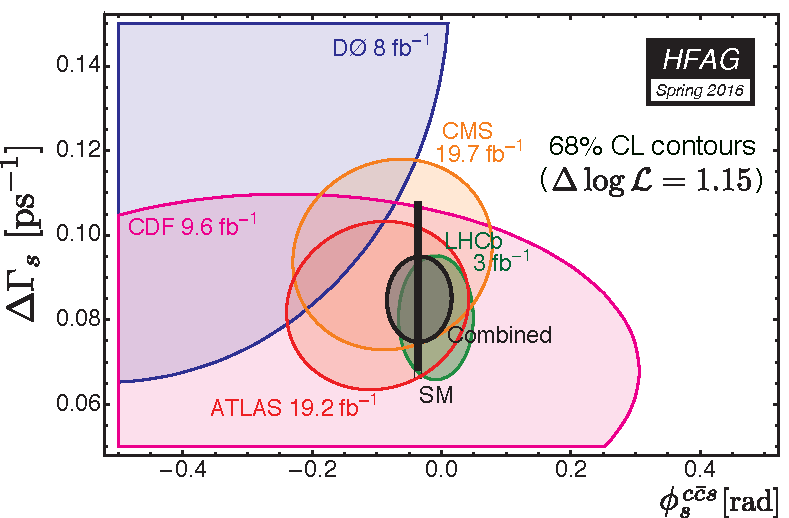
\includegraphics[trim=0cm 0cm 0cm 0cm, clip=true, scale=0.8]{Figures/Chapter1/hfag_Spring2016_DGsphis_zoom.pdf}
    \caption{Likelihood contours of $\Delta\Gamma-\phis$ (here $\phis\equiv \phis^{c\bar{cs}}$). Many individual measurements are
             combined to the black elipse. Standard Model prediction is represented by the black band. The \lhcb measurement
             mentioned in \equref{} is illustrated by the green elipse. The combined measurements agree with the Standard Model
             predictions. Plot from \cite{HFAG} {\color{red} cite hfag} }
    \label{hfag_phis_dg}
  \end{center}
\end{figure}

\begin{subequations}
  \begin{align}
  \centering
  \phiS{\lhcb}           &=  -0.010 \pm 0.039(\text{total})  \;\; \text{rad}
  \label{phis_lhcb} \\
  \phiS{SM,tree}  &=  -2\betas = -0.0376 {}^{+0.0008}_{-0.0007}  \;\; \text{rad}
  \label{phis_theo}
\end{align}
\end{subequations}

The status of the \phis measurements is shown in \figref{hfag_phis_dg}, where \lhcb has the most precise measurement to date.
The combined \phis value from the \lhcb experiment {\color{red} cite phiscombi} is shown in \equref{phis_lhcb}.
The last agrees with the Standard Model of \equref{phis_theo}, predictions within the current experimental ucertainty.
